\section{Synthetic Data Engine and Dynamic Equilibrium}
\label{sec:data-engine}

\subsection{Rationale for a Controlled Generator}

Evaluating a spillover-aware estimator on observational urban data is
circular: the spillover structure is exactly what is unknown, so a model that
appears to exploit it cannot be distinguished from one that has fit
confounding. We therefore evaluate primarily on a synthetic city whose
data-generating process we specify completely. This licenses the question that
motivates the paper---\emph{when spillover is known to be present, does the
graph model recover it?}---and, as Section~\ref{subsec:collapse} shows, the
answer is not automatically yes.

\subsection{Graph and State Variables}

The synthetic city is a $4 \times 4$ lattice of $N = 16$ neighbourhood units
with four-connected adjacency, giving $|E| = 48$ directed edge entries and
degrees between two and four. Each unit carries the six state variables of
Section~\ref{sec:methodology}, initialised with multiplicative Gaussian
heterogeneity around city-wide bases (land value $100$, rent $50$, population
$2000$, median income $60{,}000$, housing units $900$, accessibility $1.0$).
Generation is fully seeded and reproducible.

Dynamics are deliberately transparent. Accessibility shocks raise land values;
land value growth feeds rent growth with a one-step lag; rent pressure damps
population, income and housing growth; and neighbour terms diffuse land and
rent across edges. A designated shock set $S = \{0,1,4,7\}$ receives a permanent
accessibility uplift from $t \geq 3$, representing a transit investment.

\subsection{The Static Intercept Collapse}
\label{subsec:collapse}

Our first generator used only that permanent shock. Under it, every model we
tested failed to benefit from the graph. The Spatial Lag Model's learned
spatial coefficient converged to $\rho \approx 0$ across seeds
($-0.05$, $-0.07$, $0.02$); \CGCEN{} with edges removed was \emph{better} than
with the real graph ($14.16$ versus $14.82$ MAE); and randomly rewiring the
edges was statistically indistinguishable from the true topology
($p = 0.70$--$0.93$).

The mechanism is instructive. A permanent shock applied at $t = 3$ to a fixed
node set means that, by the evaluation window at $t \geq 12$, each unit's
neighbour contribution has converged to a time-invariant constant. That
constant is absorbed into the unit's own level and is recovered perfectly by
the residual anchor $X_{i,t}$ in \eqref{eq:decomposition}. In other words,
spillover that is both permanent and early is observationally equivalent to a
node-specific fixed effect. There is nothing for a graph to contribute, because
the information has already been encoded in the ego trajectory. We call this
\emph{static intercept collapse}. It is, we suspect, a common and under-reported
failure mode in spatio-temporal benchmarks that inject spillover as a one-time
regime change.

\subsection{Dynamic Network Shocks}

The remedy is to make the spillover process genuinely dynamic. We augment the
generator with stochastic, recurrent accessibility pulses. At each step every
unit independently receives a pulse with probability $p_{\mathrm{pulse}} =
0.22$, of magnitude drawn uniformly from $[0.5\,\sigma_p,\, 1.5\,\sigma_p]$
with $\sigma_p = 1.2$:
\begin{equation}
  u_{i,t} \sim \mathrm{Bernoulli}(p_{\mathrm{pulse}}) \cdot
                \mathcal{U}(0.5\sigma_p,\, 1.5\sigma_p).
  \label{eq:pulse}
\end{equation}
The pulse enters the unit's own observed accessibility at $t$, and---this is
the essential coupling---transmits to \emph{neighbours'} rent growth at $t+1$:
\begin{equation}
  g^{\mathrm{rent}}_{i,t} \mathrel{+}= \lambda_p \sum_{j \in \mathcal{N}(i)}
  W_{ij} \, u_{j,t-1},
  \label{eq:pulse-transmission}
\end{equation}
with transmission strength $\lambda_p = 0.22$.

Because the pulse is transient and stochastic, a neighbour's pulse at $t$
cannot be inferred from unit $i$'s own history: it is new information available
only across an edge. This is what makes the graph necessary rather than merely
available. Accessibility is an observed feature, so the neighbour's pulse is
visible to a message-passing model at $t$ and predictive of ego rent at $t+1$,
while remaining invisible to any purely node-local estimator.

\subsection{Logistic Carrying Capacities and Bounded Trajectories}

The original generator applied purely multiplicative growth with no
equilibrating force, which produced a second and more damaging defect. Rents
compounded without bound; as the rent-to-income ratio grew, the income update's
rent-pressure term drove income sharply negative; and income collided with its
hard floor. In the unmodified generator, income reached the floor at $t = 52$
and by $t = 100$ \emph{all sixteen units were pinned at it} while mean rent had
compounded to $\approx 4 \times 10^{10}$. Any statistic computed beyond
$t \approx 52$ measured the clamp function, not the economy.

We introduce a logistic carrying-capacity structure. Each growth rate is
multiplied by a headroom factor that vanishes as the state approaches its
capacity,
\begin{equation}
  \mathrm{headroom}(x, K) = \max\!\left(0,\; 1 - \frac{x}{K}\right),
  \label{eq:headroom}
\end{equation}
with land capacity $K_L = 12 \times$ base land value, income capacity
$K_Y = 4 \times$ base income, and a rent capacity tied to contemporaneous
ability to pay, $K_R = 0.012 \times \mathrm{Income}_{i,t-1}$. Rent and income
additionally carry mean-reversion terms pulling them toward
$0.55\,K_R$ and toward base income respectively, with rates $0.05$ and $0.02$.

The economic interpretation is a supply response: as rents approach the local
affordability ceiling, further growth is choked off by construction, vacancy
and out-migration. The numerical effect is that the synthetic economy reaches a
dynamic equilibrium rather than diverging. Under the revised generator
\emph{no unit reaches any hard state floor through $t = 100$}: mean rent
settles at $\approx 1.6 \times 10^{3}$, income at $\approx 1.5 \times 10^{5}$
and $\HT$ at $\approx 0.011$. Figure~\ref{fig:trajectories} shows the resulting
trajectories.

\subsection{Policy Scenarios}

We define four scenarios, applied to the shock-node boundary $S$ as an
intervention on the generated panel. All are deliberately simple and additive
so that their ground-truth direction is unambiguous.

\begin{itemize}
  \item \textbf{Baseline.} No intervention. Provides the untreated
  counterfactual against which all contrasts are computed.

  \item \textbf{Market-Led Development.} Upzoning without affordability
  conditions: land values rise by $4\%$ and rents by $6\%$ per unit intensity
  from $t \geq 2$. Expected to \emph{increase} displacement pressure.

  \item \textbf{Inclusionary Housing.} A mandate coupling new development to
  affordable set-asides: rents fall by $6\%$ and housing stock rises by $8\%$
  per unit intensity from $t \geq 1$. Expected to \emph{reduce} pressure.

  \item \textbf{Land-Value Capture.} Taxation of land-value uplift recycled
  into affordability: land values rise by a damped $2\%$ while rents fall by
  $5\%$ per unit intensity from $t \geq 2$. Expected to reduce pressure, with a
  different land/rent signature from inclusionary housing.
\end{itemize}

Scenario intensities ($0.8$, $0.6$, $0.7$ respectively) are configuration
parameters, not fitted quantities. For each of ten seeds we export all four
scenario panels together with adjacency, edge index, low-income share and the
treated boundary, giving $10 \times 4 = 40$ reproducible datasets.

\begin{figure*}[t]
  \centering
  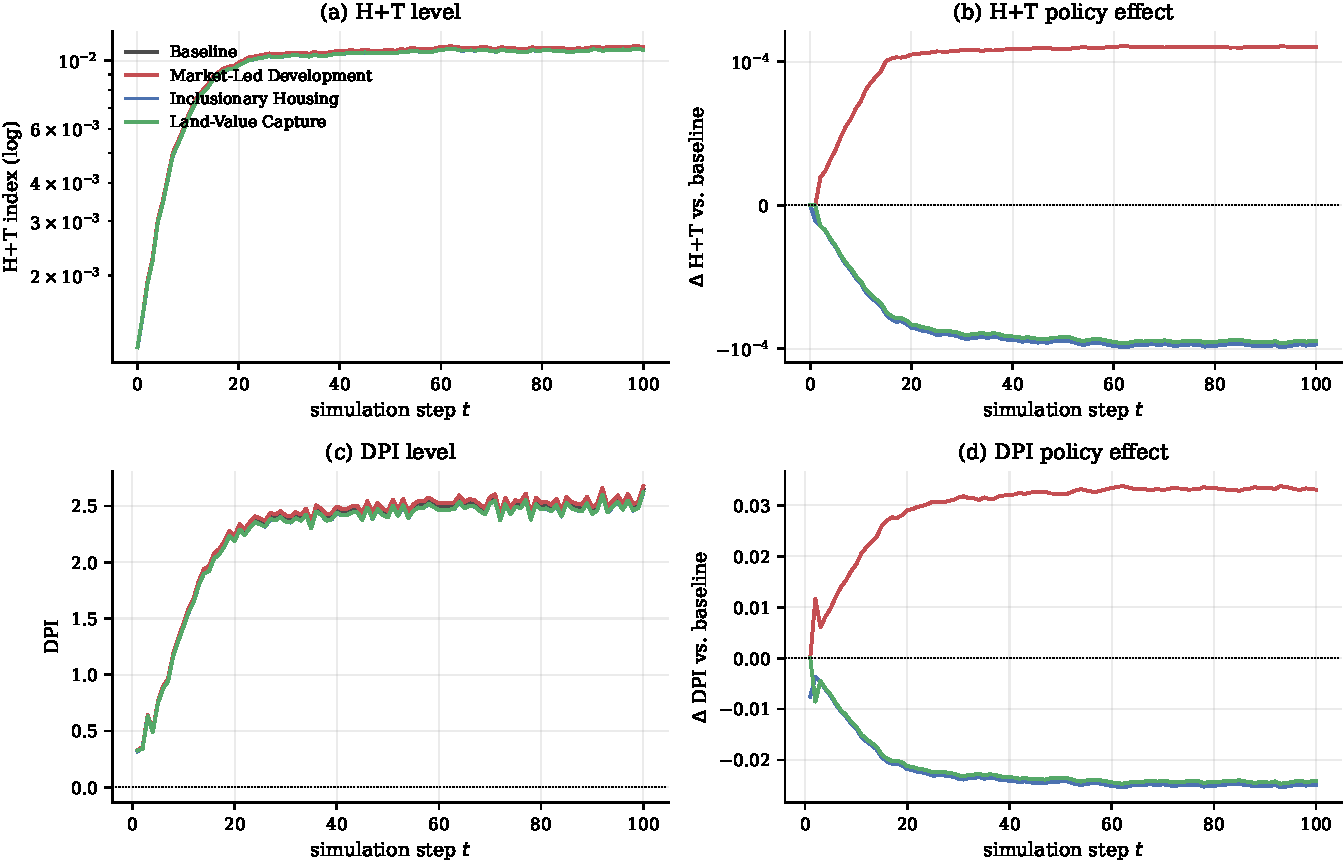
\includegraphics[width=\textwidth]{scenario_trajectories.pdf}
  \caption{Scenario trajectories over $t = 0 \dots 100$ (city-mean, seed 1).
  Panels (a) and (c) show $\HT$ and $\DPI$ levels; panels (b) and (d) show each
  intervention relative to the untreated baseline, which is the comparative
  quantity of interest. Under the logistic carrying capacities and mean
  reversion of \eqref{eq:headroom}, the economy reaches a dynamic equilibrium
  and no unit reaches a hard state floor over the full horizon. Policy effects
  persist as sustained level offsets rather than the single-step transients
  produced by a growth-rate-only index.}
  \label{fig:trajectories}
\end{figure*}
